 \iffalse
\let\negmedspace\undefined
\let\negthickspace\undefined
\documentclass[journal,12pt,twocolumn]{IEEEtran}
\usepackage{cite}
\usepackage{amsmath,amssymb,amsfonts,amsthm}
\usepackage{algorithmic}
\usepackage{graphicx}
\usepackage{textcomp}
\usepackage{xcolor}
\usepackage{txfonts}
\usepackage{listings}
\usepackage{enumitem}
\usepackage{mathtools}
\usepackage{gensymb}
\usepackage{comment}
\usepackage{tikz}
\usepackage[breaklinks=true,hidelinks]{hyperref}
\usepackage{tkz-euclide} 
\usepackage{listings}
\usepackage{gvv}
\def\inputGnumericTable{}
\usepackage[latin1]{inputenc}                              
\usepackage{color} 
\usepackage{array}                                            
\usepackage{longtable}                                       
\usepackage{calc}                                             
\usepackage{multirow}                                         
\usepackage{hhline}                                           
\usepackage{ifthen}                                           
\usepackage{lscape}

\newtheorem{theorem}{Theorem}[section]
\newtheorem{problem}{Problem}
\newtheorem{proposition}{Proposition}[section]
\newtheorem{lemma}{Lemma}[section]
\newtheorem{corollary}[theorem]{Corollary}
\newtheorem{example}{Example}[section]
\newtheorem{definition}[problem]{Definition}
\newcommand{\BEQA}{\begin{eqnarray}}
\newcommand{\EEQA}{\end{eqnarray}}
\newcommand{\define}{\stackrel{\triangle}{=}}
\theoremstyle{remark}
\newtheorem{rem}{Remark}
\begin{document}

\bibliographystyle{IEEEtran}
\vspace{3cm}

\title{GATE 2021 BM Q-31}
\author{EE23BTECH11207 -KAILASH.C$^{*}$% <-this % stops a space
}
\maketitle
\newpage
\bigskip

\renewcommand{\thefigure}{\theenumi}
\renewcommand{\thetable}{\theenumi}
In the block diagram shown below, an infinite tap FIR filter with transfer function $H\brak{z}=\frac{Y\brak{z}}{X\brak{z}}$ is realized. If $H\brak{z}=\frac{1}{1-0.5z^{-1}}$.\\the value of $\alpha$ is
\begin{figure}[h]
    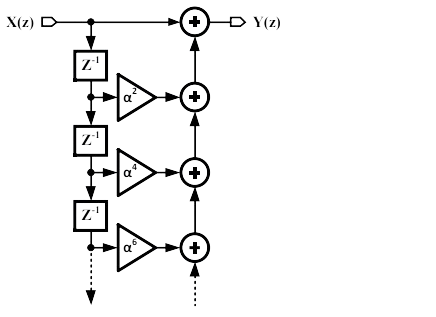
\includegraphics[width=1\columnwidth]{2021/BM/31/figs/questionfig.png}
    \label{fig:question31bm}
\end{figure} \hfill(GATE 2021 BM)\\
\solution
\fi
\begin{table}[h]
\begin{tabular}{|l|l|l|}
\hline
\textbf{Parameter} & \textbf{Definition}\\ \hline
$H\brak{z} & $\frac{1}{1-0.5z^{-1}}$ \\ \hline
\end{tabular}
\caption{Parameter Table}
\label{tab:gate.bm.31.2021}
\end{table}
\\
From diagram we have:
\begin{align}
    Y\brak{z}&=X\brak{z}\brak{\sum_{n=0}^{\infty}\brak{z^{-1}\alpha^{2}}^n}\label{eq:311_bm}
\end{align}
Dividing by $X\brak{z}$ in both sides:
\begin{align}
    \frac{Y\brak{z}}{X\brak{z}}&=\sum_{n=0}^{\infty}\brak{z^{-1}\alpha^{2}}^n\label{eq:312_bm}\\
    \implies H\brak{z}&=\sum_{n=0}^{\infty}\brak{z^{-1}\alpha^{2}}^n\label{eq:313_bm}\\
    \frac{1}{1-0.5z^{-1}}&=\sum_{n=0}^{\infty}\brak{z^{-1}\alpha^{2}}^n\label{eq:314_bm}\\
\frac{1}{1-0.5z^{-1}}&=\frac{1}{1-z^{-1}\alpha^{2}}\label{eq:315_bm}\\
\implies \alpha&=\frac{1}{\sqrt{2}}\label{eq:316_bm}
\end{align}
